\subsection{Sequence-to-SQL}

\subsubsection{Seq2Seq}

In natural language processing, Sequence-to-Sequence (Seq2Seq)\cite{DBLP:journals/corr/SutskeverVL14} models are a type of neural network architecture used for tasks such as machine translation, text summarization, and text-to-speech conversion. These are the two main components of the model. Encoders and decoders make up the core of the Seq2Seq model. The encoder receives a stream of data as input, such as a sentence written in one language, and transforms it into a representation with a fixed length, which is also referred to as the hidden state. This concealed state is then sent to the decoder, which is responsible for generating the output sequence, which may include the sentence being translated into a different language.

There are a variety of methods that can be used to train Seq2Seq models, such as supervised learning, in which the model is trained on a dataset of input-output pairs, and unsupervised learning, in which the model is trained to reconstruct the input sequence. Both of these methods are examples of how the model can be trained. Attention mechanisms, such as the attention mechanism used in the Transformer model, can also be incorporated into Seq2Seq models to improve their performance. This is accomplished by allowing the decoder to focus selectively on certain parts of the input sequence. Attention mechanisms can also be used in the Transformer model.

Natural language processing applications make extensive use of Seq2Seq models because of their versatility in managing sequences of varying lengths, both in terms of input and output and also in terms of the data they process sequentially. However, one of the most significant difficulties associated with Seq2Seq models is the possibility of producing outputs that are irrelevant or need to be clarified. This issue is referred to as the "exposure bias" problem. Researchers have come up with several potential solutions to this issue, including using beam search while the model is being trained or training the model with scheduled sampling.

% image of seq2seq.png
\begin{figure}[ht]
    \centering
    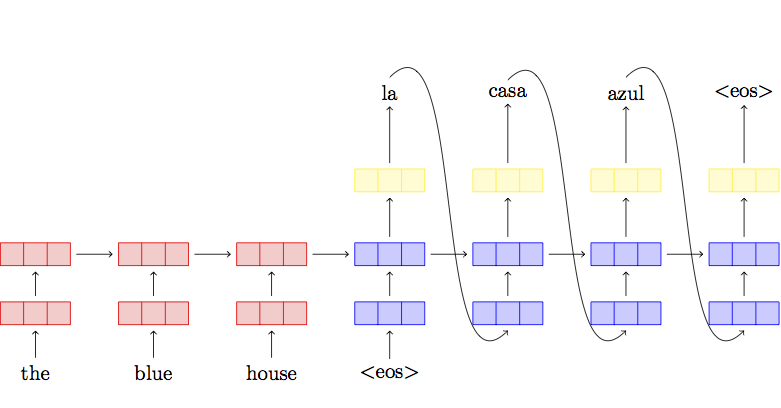
\includegraphics[width=0.5\textwidth]{pics/seq2seq.png}
    \caption{Example of Seq2Seq model in translating a sentence from English to French.}
    \label{fig:seq2seq}
\end{figure}

\subsubsection{Seq2SQL}

An output of a sequence-to-sequence approach is a sequence of SQL tokens and schema elements, with that sequence being used to predict SQL queries or at least a significant portion of them. An NLQ sequence is transformed into a SQL sequence by these programs. There is no doubt that this approach is the simplest, but it is also the most error-prone. Seq2SQL\cite{zhong_seq2sql_2017}, one of the first deep-learning systems, used this approach, but later, systems avoided it. sequence-to-sequence architectures have the major disadvantage of not taking the strict grammar rules of SQL into account when generating queries.

As part of this model, its authors released the WikiSQL dataset, which ushered in a new era of text-to-SQL deep learning research. GloVe embeddings represent the inputs in the network architecture, which combines LSTM and linear layers. With a seq-to-seq network, the system predicts the aggregation function and the column for the SELECT clause. Its major drawback is that it generates parts of the query that can lead to syntactic errors.